\documentclass[lualatex,handout]{beamer}
\setbeamertemplate{footline}[frame number]
\usepackage{luatexja}
\usepackage{amsmath,amssymb}

\usepackage{thm-restate}

%\usetheme{Berlin}
\usecolortheme{rose}

\usepackage{tikz}
\usepackage{pgfplots}
\pgfplotsset{compat=1.18}

%\usepackage[haranoaji]{luatexja-preset}
\usepackage[deluxe,ipaex]{luatexja-preset}
\renewcommand{\kanjifamilydefault}{\gtdefault}
%\setmainjfont{HaranoAjiGothic-Regular}

\usepackage{unicode-math}
%\setmathfont{Fira Math}
\setmathfont{STIX Two Math}
\setmathfont{STIX Two Math}[range=bfup/{Latin,latin,num,Greek,greek}]
\setmathfont{STIX Two Math}[range=bfit/{Latin,latin}]
\setmathfont{STIX Two Math}[range={"0000-"FFFF}]
\setmathrm{STIX Two Math}[StylisticSet=8]

%\usefonttheme{professionalfonts}

\usepackage{luacolor}

\newcommand{\mycolor}[2]{%
  \begingroup
  \colorlet{currentcolor}{.}%
  \color{#1}#2%
  \color{currentcolor}%
  \endgroup
}
\newcommand{\emm}[1]{\mycolor{red}{#1}}
\newcommand{\expt}[1]{\mathbb{E}\left[#1\right]}
\newcommand{\var}[1]{\mathbb{V}\left[#1\right]}
\newcommand{\cov}[1]{\mathsf{Cov}\left[#1\right]}
\newcommand{\vc}[1]{\mathsf{Var}\left[#1\right]}

\DeclareMathOperator*{\argmax}{arg\,max}


\usepackage{xspace}
%\usepackage{bm}
%\newcommand\bm[1]{{\mathbf{#1}}}
\newcommand\defiff{\stackrel{\text{def}}{\iff}}
\newcommand\dx{{\,\mathrm{d}x}}
\newcommand\KL[2]{D\left(#1\,\|\,#2\right)}
\newcommand\dtv{d_{\mathrm{TV}}}

\theoremstyle{definition}

\title{確率・統計基礎: 仮説検定}
\author{森 立平}
\date{}



\begin{document}
\begin{frame}[plain]
\maketitle
\end{frame}


\begin{frame}{仮説検定}
答が\emm{二値}の推定問題を考えたいが\emm{事前分布を適切に決める方法がない}。

\vspace{3em}
\begin{itemize}
\setlength{\itemsep}{2em}
\item 開発中の薬に効果があるかないか。
\item 患者が病気かどうか。
\end{itemize}
\end{frame}

\begin{frame}{仮説検定}
\begin{itemize}
\setlength{\itemsep}{2em}
\item 対立仮説
\item 帰無仮説
\end{itemize}
\end{frame}

\begin{frame}{数学的な問題設定}
\small

以下では$s=0$が帰無仮説、$s=1$が対立仮説に対応しているとする。

検定関数$E\colon A\to\{0,1\}$は$E(x)=0$のとき帰無仮説を採択、$E(x)=1$のとき帰無仮説を棄却することを表す。
以下では\emm{確率的な検定関数}$E\colon A\to [0,1]$を考える。$E(x)\in[0,1]$は帰無仮説を\emm{棄却する確率}を表す。

\begin{block}{問題}
尤度関数$\Pr(X = x\mid S=s)$が既知である。
与えられた$x\in A$から$s\in \{0,1\}$を推定したい。
検定関数$E\colon A\to \{0,1\}$の
第一種誤り確率は$\alpha_E\coloneq\Pr(E(X) = 1\mid S= 0)$、
第二種誤り確率は$\beta_E\coloneq\Pr(E(X) = 0\mid S= 1)$
で定義される。
\end{block}

\vspace{2em}
第一種誤り確率を小さくしたければ$E(x) = 0$とすればよいし
第二種誤り確率を小さくしたければ$E(x) = 1$とすればよい。

\end{frame}

\begin{frame}{二種類の誤り確率}
\centering
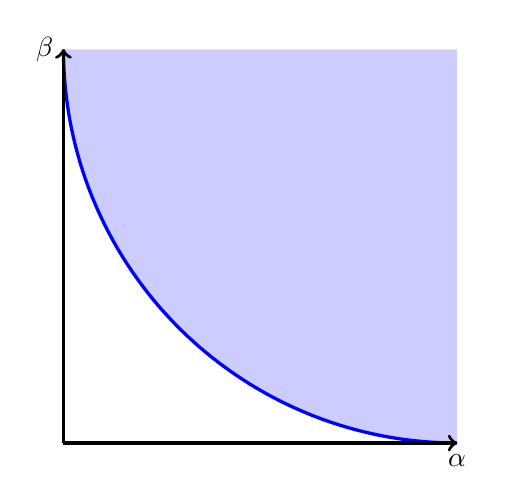
\begin{tikzpicture}
  \fill[blue!20, domain=180:270, samples=100] plot ({5*cos(\x) + 5}, {5*sin(\x) + 5}) -- (5,5) -- cycle;
  
  \draw[thick, blue, domain=180:270, samples=100, very thick] plot ({5*cos(\x)+5}, {5*sin(\x)+5}) node[right] {};

  \draw[->,very thick] (-0,0) -- (5,0) node[below] {$\alpha$};
  \draw[->,very thick] (0,-0) -- (0,5) node[left] {$\beta$};
\end{tikzpicture}

実現可能な$(\alpha_E,\beta_E)$の集合
\begin{align*}
\left\{(\alpha_E,\beta_E)\mid E\right\}
\end{align*}
は凸集合である。

二つの検定関数$E_1$と$E_2$の確率混合$\lambda E_1(x) + (1-\lambda) E_2(x)$は
\end{frame}

\begin{frame}{尤度比検定}
事前分布が分かっている場合、
\begin{align*}
E_{\mathrm{MAP}}(x)&=
\begin{cases}
0&\text{if } \frac{\Pr(X = x\mid S = 0)}{\Pr(X = x\mid S = 1)} \ge \frac{\Pr(S = 1)}{\Pr(S = 0)}\\
1&\text{otherwise.}
\end{cases}
\end{align*}
が最適な検定関数となる。

\vspace{2em}
一般的に
\begin{align*}
E_{\eta}(x)&=
\begin{cases}
0&\text{if } \frac{\Pr(X = x\mid S = 0)}{\Pr(X = x\mid S = 1)} \ge \eta\\
1&\text{otherwise.}
\end{cases}
\end{align*}
という形の検定関数を用いた仮説検定を\emm{尤度比検定}という。
\end{frame}

\begin{frame}{ネイマン・ピアソンの補題}
\begin{definition}[最強力検定]
%検定関数$E\colon A\to \{0,1\}$が有意水準$\alpha\in[0,1]$の最強力検定であるとは以下を満たすことである。
%\begin{enumerate}
%\item $\alpha_E = \alpha$.
%\item $\beta_E = \min\{ \beta_{E'}\mid E', \alpha_{E'}\ge \alpha\}$.
%\end{enumerate}
検定関数$E\colon A\to \{0,1\}$がの最強力検定$\defiff$
任意の$E'$について$\alpha_{E'}\ge \alpha_E$もしくは$\beta_{E'}\ge \beta_E$が成り立つ。
\end{definition}
\begin{lemma}[ネイマン・ピアソンの補題]
%任意の$\alpha\in[0,1]$について、ある$\eta\in\mathbb{R}$が存在し、$E_\eta$は最強力検定である。
任意の$\eta\in\mathbb{R}$について$E_\eta$は最強力検定である。
\end{lemma}
\begin{proof}
$L\coloneq\left\{x\in A\mid \frac{p_0(x)}{p_1(x)}\ge \eta\right\}$とおくと、
\begin{align*}
(E(x) - E'(x)) (p_0(x) - \eta p_1(x))&\ge 0
\end{align*}
\end{proof}
\end{frame}


\begin{frame}{課題}
\small
$A=\{0,1,2\},\,B=\{0, 1\}$とし、
\begin{align*}
\Pr(S = 0) &= 1/4&
\Pr(S = 1) &= 3/4\\
\Pr(X=0\mid S=0) &= 1/6&
\Pr(X=1\mid S=0) &= 2/6&
\Pr(X=2\mid S=0) &= 3/6\\
\Pr(X=0\mid S=1) &= 3/6&
\Pr(X=1\mid S=1) &= 1/6&
\Pr(X=2\mid S=1) &= 2/6\\
\end{align*}
とするとき、以下の問に答えよ。
\vspace{1em}
\begin{enumerate}
\setlength{\itemsep}{1em}
\item $X$から$S$を最大事後確率推定する関数$E_{\mathrm{MAP}}\colon A\to B$と最尤推定する関数$E_{\mathrm{ML}}\colon A\to B$をもとめよ。
%事後確率や尤度が等しい場合ものが複数ある場合は一様に選ぶことにせよ。
\item $X$から$S$を最大事後確率推定した場合の平均誤り確率をもとめよ。
\item $X$から$S$を最尤推定した場合の平均誤り確率をもとめよ。
\end{enumerate}
\end{frame}

\if0
\begin{frame}{おまけ 1/2}
\footnotesize
\begin{definition}[対称通信路]
$B=\{0,1\}$とする。
通信路$\Pr(X=s\mid S=s)$についてある置換$\sigma\colon A\to A$が存在して
$\sigma^2=\mathrm{id}$で
\begin{align*}
\Pr(X = x\mid S = 0) &= \Pr(X = \sigma(x)\mid S = 1)
\end{align*}
が成り立つとき$\Pr(X=x\mid S=s)$を\emm{対称通信路}という。
\end{definition}
$\lambda=1/2$と$\Pr(X=x\mid S=s)$が対称通信路であることを仮定すると、
\begin{align*}
&\lambda \Pr\left(\emm{\sum_{k=1}^N \log\frac{p(X_k\mid 0)}{p(X_k\mid 1)}} \le \log\frac{1-\lambda}{\lambda}\mid S=0\right)\\
&\quad + (1-\lambda) \Pr\left(\emm{\sum_{k=1}^N \log\frac{p(X_k\mid 1)}{p(X_k\mid 0)}} \le \log\frac{\lambda}{1-\lambda}\mid S=1\right)\\
&=
\frac12 \Pr\left(\emm{\sum_{k=1}^N \log\frac{p(X_k\mid 0)}{p(X_k\mid 1)}} \le 0\mid S=0\right)
+ \frac12 \Pr\left(\emm{\sum_{k=1}^N \log\frac{p(X_k\mid 1)}{p(X_k\mid 0)}} \le 0\mid S=1\right)\\
&=
\frac12 \Pr\left(\emm{\sum_{k=1}^N \log\frac{p(X_k\mid 0)}{p(X_k\mid 1)}} \le 0\mid S=0\right)
+ \frac12 \Pr\left(\emm{\sum_{k=1}^N \log\frac{p(\sigma(\sigma(X_k))\mid 0)}{p(\sigma(\sigma(X_k))\mid 1)}} \le 0\mid S=0\right)\\
&=
\Pr\left(\emm{\sum_{k=1}^N \log\frac{p(X_k\mid 0)}{p(X_k\mid 1)}} \le 0\mid S=0\right).
\end{align*}
\end{frame}

\begin{frame}{おまけ 2/2}
$Y=\log\frac{p(X\mid 1)}{p(X\mid 0)}$とすると、任意の$t\ge 0$について
\begin{align*}
\Pr\left(\emm{\sum_{k=1}^N \log\frac{p(X_k\mid 0)}{p(X_k\mid 1)}} \le 0\mid S=0\right)
&=\Pr\left(\emm{\sum_{k=1}^N \log\frac{p(X_k\mid 1)}{p(X_k\mid 0)}} \ge 0\mid S=0\right)\\
&\le M_Y(t)^N.
\end{align*}
である。ここで
\begin{align*}
M_Y(t) &= \sum_{x\in A} p_0(x) \left(\frac{p_1(x)}{p_0(x)}\right)^t = \mathrm{e}^{-(1-t)D(p_1||p_0)}
\end{align*}
\begin{definition}[R\'enyi ダイバージェンス]
\begin{align*}
D_\alpha(q||p) &= \frac1{\alpha - 1} \log \sum_{x\in A} q^\alpha(x) p^{1-\alpha}(x)
\end{align*}
\end{definition}
\end{frame}
\fi

\end{document}
